%!TEX root = ../Thesis.tex

The aim of this thesis was to use enrichment analyses to identify properties of cancer cell lines that are associated with an increased sensitivity or resistance toward a certain drug. In Chapter~\ref{chapter:Mats}, we introduced the data types and sources we employed for our analyses, while Chapter~\ref{chapter:Impl} discussed our study design and implementation details. In the following, we present the results of our analysis.\\
First, we investigate genes and pathways that were associated with drug sensitivity/resistance in a large number of drugs. Next, we investigated one exemplary drug, Rapamycin, in detail to study drug-specific response markers. Finally, we performed a PCA to investigate whether we can identify subgroups of cell lines with common expression and enrichment patterns.
%We\remove{find link to Hallmarks Of Cancer, also for pathways} used several different approaches for visualisation and interpretation of the data results from the enrichment analyses we described earlier. We will start out with a simple script to count how often a certain gene or pathway (depending on the enrichment considered) was enriched or depleted. Next, we will focus on Rapamycin as a representative drug, considering the effect the enrichment analyses observed on the sensitivity to that specific drug.\\

\section{Across-drug Analysis of Enrichment and Depletion Frequency Count}\label{sec:bidir_bar_plots}
For a first step in visualising and interpreting the results of the enrichment analyses, we counted for how many drugs the up- or down-regulation of a certain gene or pathway was linked to increased sensitivity or resistance to that drug.\\
This post-processing was performed for all three of the enrichments we performed in total. We will now go over the results for each enrichment, and set them into the appropriate scientific context.\\
In the following, we will present only a subset of the investigated enrichments: in particular, we only show the results from the analyses on data from the GDSC2 database, due to the improvements in screening procedure and other aspects GDSC2 presented over its predecessor~\cite{gdsc}. Also, we only consider the CMax-Viability value, since it allows for comparison across drugs~\cite{cmax_viability}, which is what we are considering here. Results for the IC50 drug sensitivity score and the GDSC1 database can be found in \hyperref[appendix:bidir]{Appendix A}. For the enrichment analyses based on expression values, we only consider the normalization using absolute z-scores. The enrichment analyses based on the expression values themselves and the z-scores can also be found in \hyperref[appendix:bidir]{Appendix A}.
%For the purpose of this visualization, we limited ourselves in the analyses we considered. For the first and third enrichment, we had the choice between the IC50 and CMax-Viability values for the drug sensitivity, for which we selected the CMax-Viability because of the optimizations it presents in contrast to the IC50, namely it considering the most interesting drug dose (the highest clinical dose), and it being comparable across drugs~\cite{cmax_viability}. We also selected the GDSC2 database, as the team which created GDSC introduced GDSC2 as a successor to the GDSC1 database, including but not limited to the use of optimized drug sensitivity screening procedures~\cite{gdsc}.

\subsection{Gene-based Drug Sensitivity Enrichment}\label{subsec:bidir_enr1}
For the first enrichment, we used gene expression alterations as categories for an enrichment analysis based on drug sensitivity values (CMax-Viability). We had one sorted list per drug, which contained CMax-Viability values for cell lines, sorted increasingly. As results, the enrichment gave us p-values for each gene expression alteration and drug combination, expressing how strongly this specific gene expression alteration is linked to an increased sensitivity or resistance to this specific drug. Next, we counted for how many drugs this this gene was deemed significant, which means we count for how many different drugs the gene expression alteration is liked to an increased sensitivity or resistance.
\begin{figure}
    \centering
    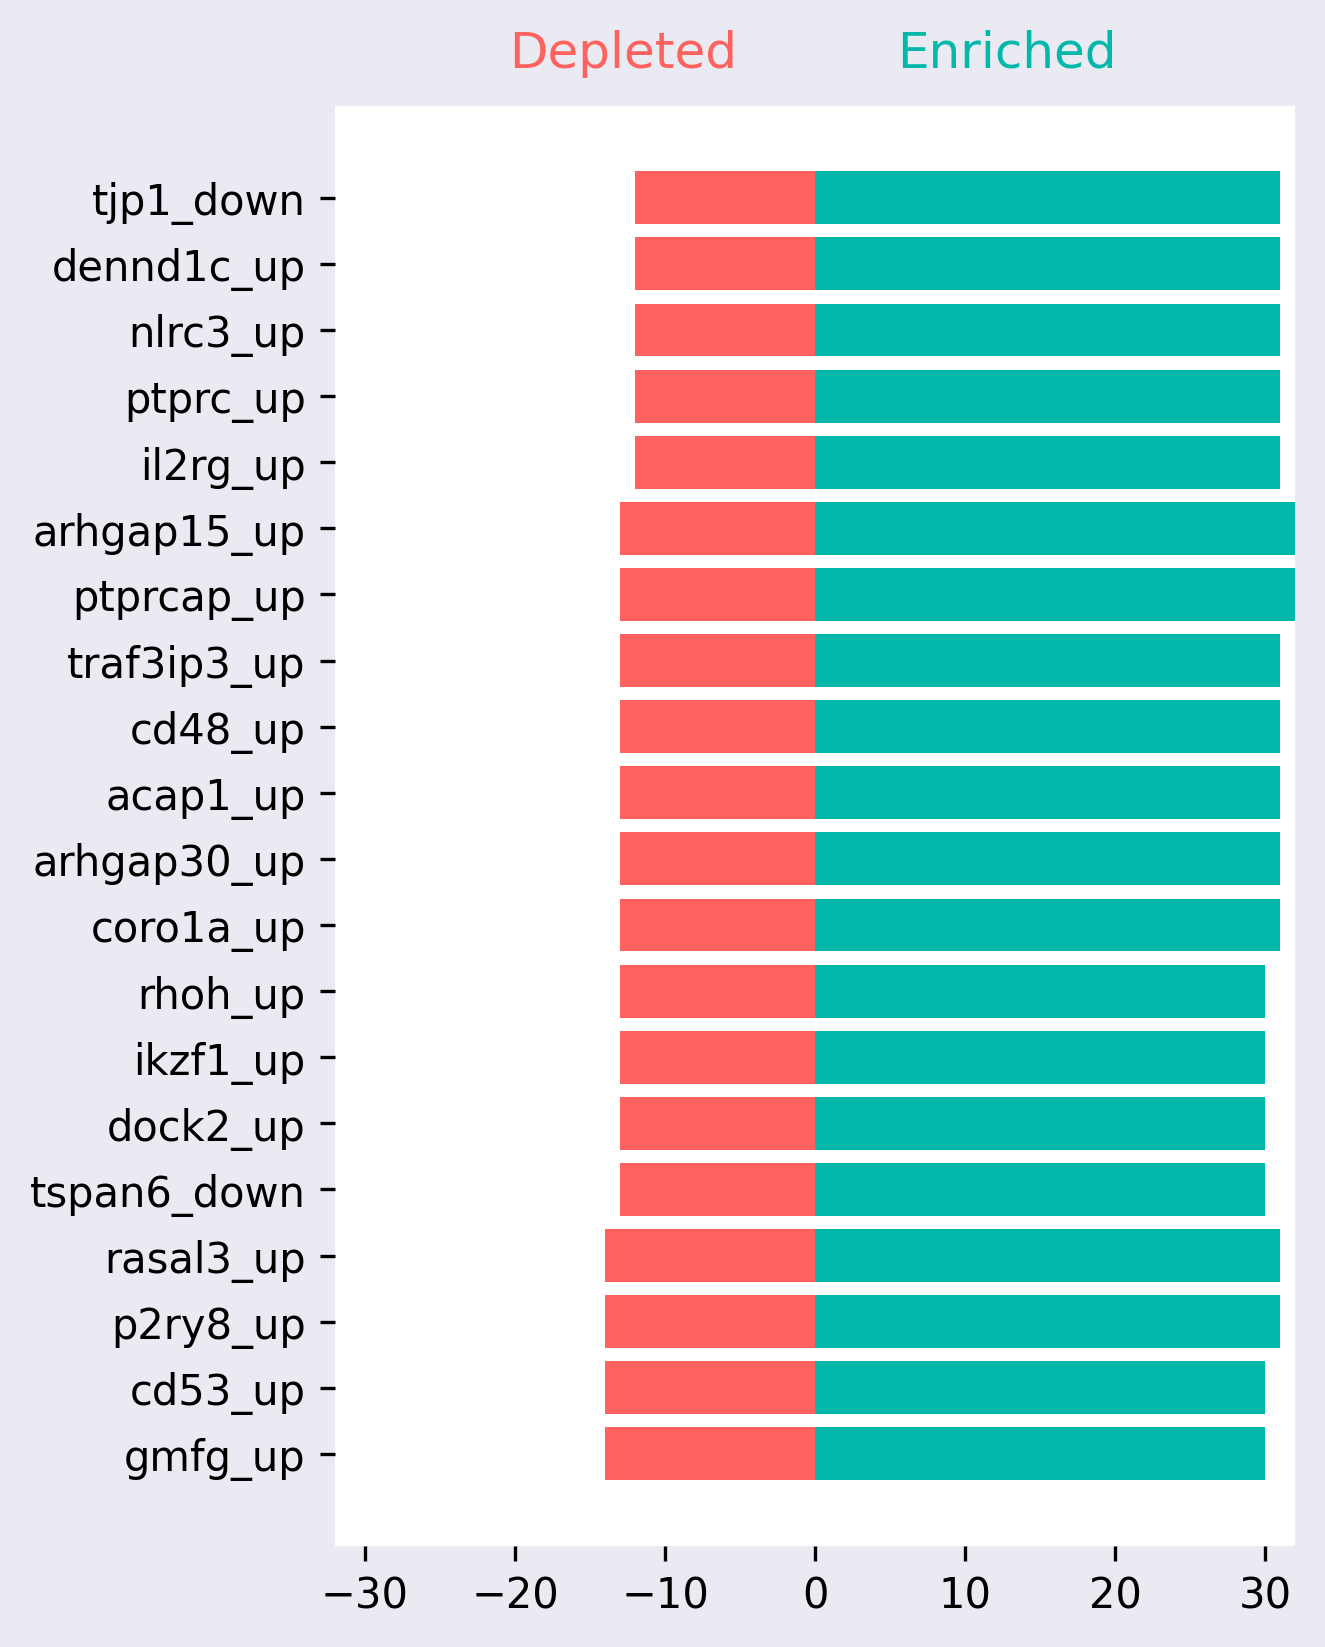
\includegraphics[width=0.5\textwidth]{bidir_bar_plot_enr1.png}
    \caption{Count of enriched and depleted genes in the gene-based drug sensitivity enrichment analysis. Count of enriched and depleted genes on $x$-axis, genes on $y$-axis. Sorted by decreasing value of $\frac{\#_{\text{enriched}}}{\#_{\text{depleted}}}$.\\Dataset: GDSC2, drug sensitivity: CMax-Viability\\The negative numbers for depleted are only there for technical reasons and still describe only the count.}
    \label{fig:bidir_enr1}
\end{figure}
The visualization of the $20$ most significant results can be found in Figure~\ref{fig:bidir_enr1}. On the left-hand side, the numbering on the x-axis is only negative for technical reasons, it should still be considered as the count of drugs for which the gene was found to be depleted.\\
Interestingly, all genes depicted in Figure~\ref{fig:bidir_enr1} were significantly enriched for some drugs, but significantly depleted for others. This shows that the same alteration can have converse effects on the drug sensitivity for different drugs, making the cell lines more sensitive to some drugs, but at the same time more resistant to others.\\
Some interesting genes were identified and set into context from this plot. We will consider several of them in the rest of this section.\\
For instance, the gene \textbf{TJP1} (tight junction protein 1) in a down-regulated manner was found to be enriched (meaning, associated with increased drug sensitivity) for $31$ drugs and depleted (associated with increased drug resistance) for $12$ drugs. TJP1 is a membrane-associated cytosolic protein important for cell-cell communication in intracellular barriers~\cite{TJP1_Lee}. In 2020, Lee et al.\ found TJP1 down-regulation to have ``induced enhanced response against anti-cancer agents, doxorubicin and gefitinib''. This matches us finding it to be associated with high sensitivity for more drugs than resistance. However, due to the complexity of cancer drugs and the multitude of roles that tight junctions play in cancer and cell interaction in general, we still find results in both directions.\\
%For instance, the gene \textbf{TIP1}\todo{TIP1 or TJP1???} in a down-regulated category was found to be significant. This gene was identified to be inhibiting the proliferation of colon cancer cells by Han et al.\ in 2012~\cite{tip1}. As this gene appears to be a tumor inhibitor in some specific cases, it is coherent to find that the down-regulation of this gene was increased in cancer cells. Aside from that, TIP1 was also found to facilitate cell migration and metastasis of breast cancer cells~\cite{tip1_metastasis}, which is a Hallmark of Cancer~\cite{hallmarks-of-cancer}\\
Another gene which was identified as being significant across multiple datasets was \textbf{NLRC3} (nucleotide-binding domain and leucine-rich repeats), in an up-regulated fashion. It caused higher sensitivity to $31$ drugs and higher resistance to $12$ drugs. It is an an inhibitory sensor of a specific kind of mTOR-pathways in cancer~\cite{nlrc3}, which we will go more in-depth about later. This means that the gene has the ability to down-regulate these specific kinds of PI3K-mTOR pathways when it detects a specific signal. In a 2022 paper, Sun et al.\ hypothesized that NLRC3 could be a therapeutic target or a potential diagnostic tumor marker, since it has been shown to promote apoptosis, inhibit proliferation and prevent inflammation, all of which are typical for cancer (see~\ref{sec:hallmarks}). With it promoting several of the organisms natural anti-cancer defense mechanisms, it being associated to an increased drug sensitivity is coherent.\\
%Its expression was found to be ``drastically reduced in the tumour tissue of patients with colorectal cancer compared to healthy tissues, highlighting an undefined potential function for this sensor in the development of cancer''~\cite{nlrc3}. This hypothesis is supported by our finding of the up-regulation of this gene being linked to an increased sensitivity against cancer drugs. NLRC3 was also found to be a regulator of cellular proliferation and apoptosis in cancer cells~\cite{nlrc3_apoptosis_proliferation}, which are both Hallmarks of Cancer~\cite{hallmarks-of-cancer}.\\
Next, we consider the \textbf{PTPRC} gene (protein tyrosine phosphatase, receptor type C), as well as the \textbf{PTPRCAP} gene (PTPRC-associated protein), which were both also up-regulated. PTPRC and PTPRCAP were found to imply higher sensitivity against $31$ and $32$, as well as higher resistance against $12$ and $13$ drug respectively. The PTPRC gene (or, more specifically, the protein it encodes), was found to be pivotal in regulating cancer drug sensitivity, by regulating CD8+ T-cell infiltration~\cite{ptprc_cd8+}. This describes a process where a specific type of cytotoxic immune cells move into and accumulate in a specific region of tissue, such as a tumour. There, they proceed to attack the tumor. In 2023, Li et al.~\cite{ptprc_cd8+} found a higher expression of PTPRC also to be linked to a better prognosis for the patient, as well as a down-regulation of PTPRC expression to be linked to an increase in cell viability. This means that the cancer cells were more likely to survive when PTPRC expression was low, which could, hypothetically speaking, imply that up-regulation of PTPRC and PTPRCAP increased drug sensitivity.\\
%Although the fact that the up-regulation of this gene was found to be linked to an increased sensitivity against cancer drugs might sound unintuitive at first when thinking like the previous argument, we can still make sense of this result:
%The up-regulation of this gene might already weaken the tumour by strengthening the natural immune response of the body against the tumour. Since it does that in a way which is not linked to the ``point of attack'' of typical cancer drugs, the effects can accumulate without issue, so the effect of the drug might be reinforced.\\
We proceed by considering the \textbf{IL2rg} gene (Interleukin 2 receptor gamma chain). It was significantly associated with sensitivity against $31$ drugs and resistance against $12$ drugs when up-regulated. It is a critical component of several interleukin receptors. It plays a vital role in immune cell signaling, and mutations of this gene are linked to severe immunodeficiency, and ``support the growth of many types of human primary tumors''~\cite{il2rg}. IL2rg was also found to have a proto-oncogenic role in colorectal cancer, influencing processes like cell proliferation and differentiation~\cite{il2rg_differentiation}, which matches with multiple of the Hallmarks of Cancer~\cite{hallmarks-of-cancer}. In a preprint version of a 2024 paper, Hu et al.\ found IL2rg to correlate with immune cell infiltration in breast cancer, while its down-regulation was found to suppress T cell activity, aiding tumor evasion of immune surveillance. This makes it show a similar effect than the previously discussed PTPRC\@. Finally, Zheng et al.\ deemed IL2rg a receptor to be a promising drug response marker for cancer~\cite{il2rg_zheng}. This gene promoting immune response makes it coherent that its up-regulation is associated with an increased drug sensitivity across drugs.\\
Lastly, we consider the \textbf{ARHGAP15} gene (Rho GTPase activating protein 15), which is a GTPase activating protein, which inactivates the Rac1 pathway~\cite{arhgap15}. Its up-regulation was associated with increased sensitiviy for $32$ drugs, and increased resistance against $13$ drugs. It was found to be a potent tumor suppressor, by inhibiting the Rac1 pathway, which in turn plays a pivotal role in the progression of breast carcinomas~\cite{arhgap15}. In contrast, this gene was also found to promote metastatic colonization in gastric cancer~\cite{arhgap15_metastasis}, which is again a Hallmark of Cancer~\cite{hallmarks-of-cancer}. The opposing nature of the two results results implies that this gene plays a complex, but highly influential role in cancer development, which makes likely to also influence drug response both ways.

To summarize, we considered different genes and their potential links to cancer and cancer drug sensitivity. While we did find a rather direct link to cancer drug sensitivity for some of the genes, such a link was not as immediately apparent or previously documented for other genes. However, we were able to at least find a link to cancer development and aggressiveness for most genes. This could be linked to drug response, since more aggressive tumours could tend towards being more resistant to more drugs.

\subsection{Pathway-based Gene Expression Enrichment}\label{subsec:bidir_enr2}
In our second enrichment analysis, we considered a sorted list of gene expression values for every cell line instead of one for every drug, which we normalized by calculating the absolute z-scores. The list contained a sorted list of (normalized) gene expression values. For the categories, we used pathways from the KEGG database~\cite{kegg_website}. The aim of this enrichment was to identify which biological pathways were deregulated in which cancer cell lines.\\
It is important to note that the identification of altered pathways is not done in a comparative procedure to healthy cancer cells. This procedure only considers cancer cell line datasets, and calculates whether the genes belonging to the pathway are over- or underexpressed, in comparison to the genes which do not belong to the pathway. We used absolute z-scores for normalization because the up-regulation of an individual gene can have diverse effects on the regulation of the pathway it is part of, so we cannot conclude anything about the regulation direction of the pathway just from genes in the pathway being up- or downregulated~\cite{systems_biology_biological_circuits}.\\
This enrichment analysis provides a p-value for every combination of pathway and cell line, expressing how much that pathway is deregulated in that cell line, with no notion of regulation direction (cf.\ Figure~\ref{fig:bidir_enr2}).\\
\begin{figure}
    \centering
    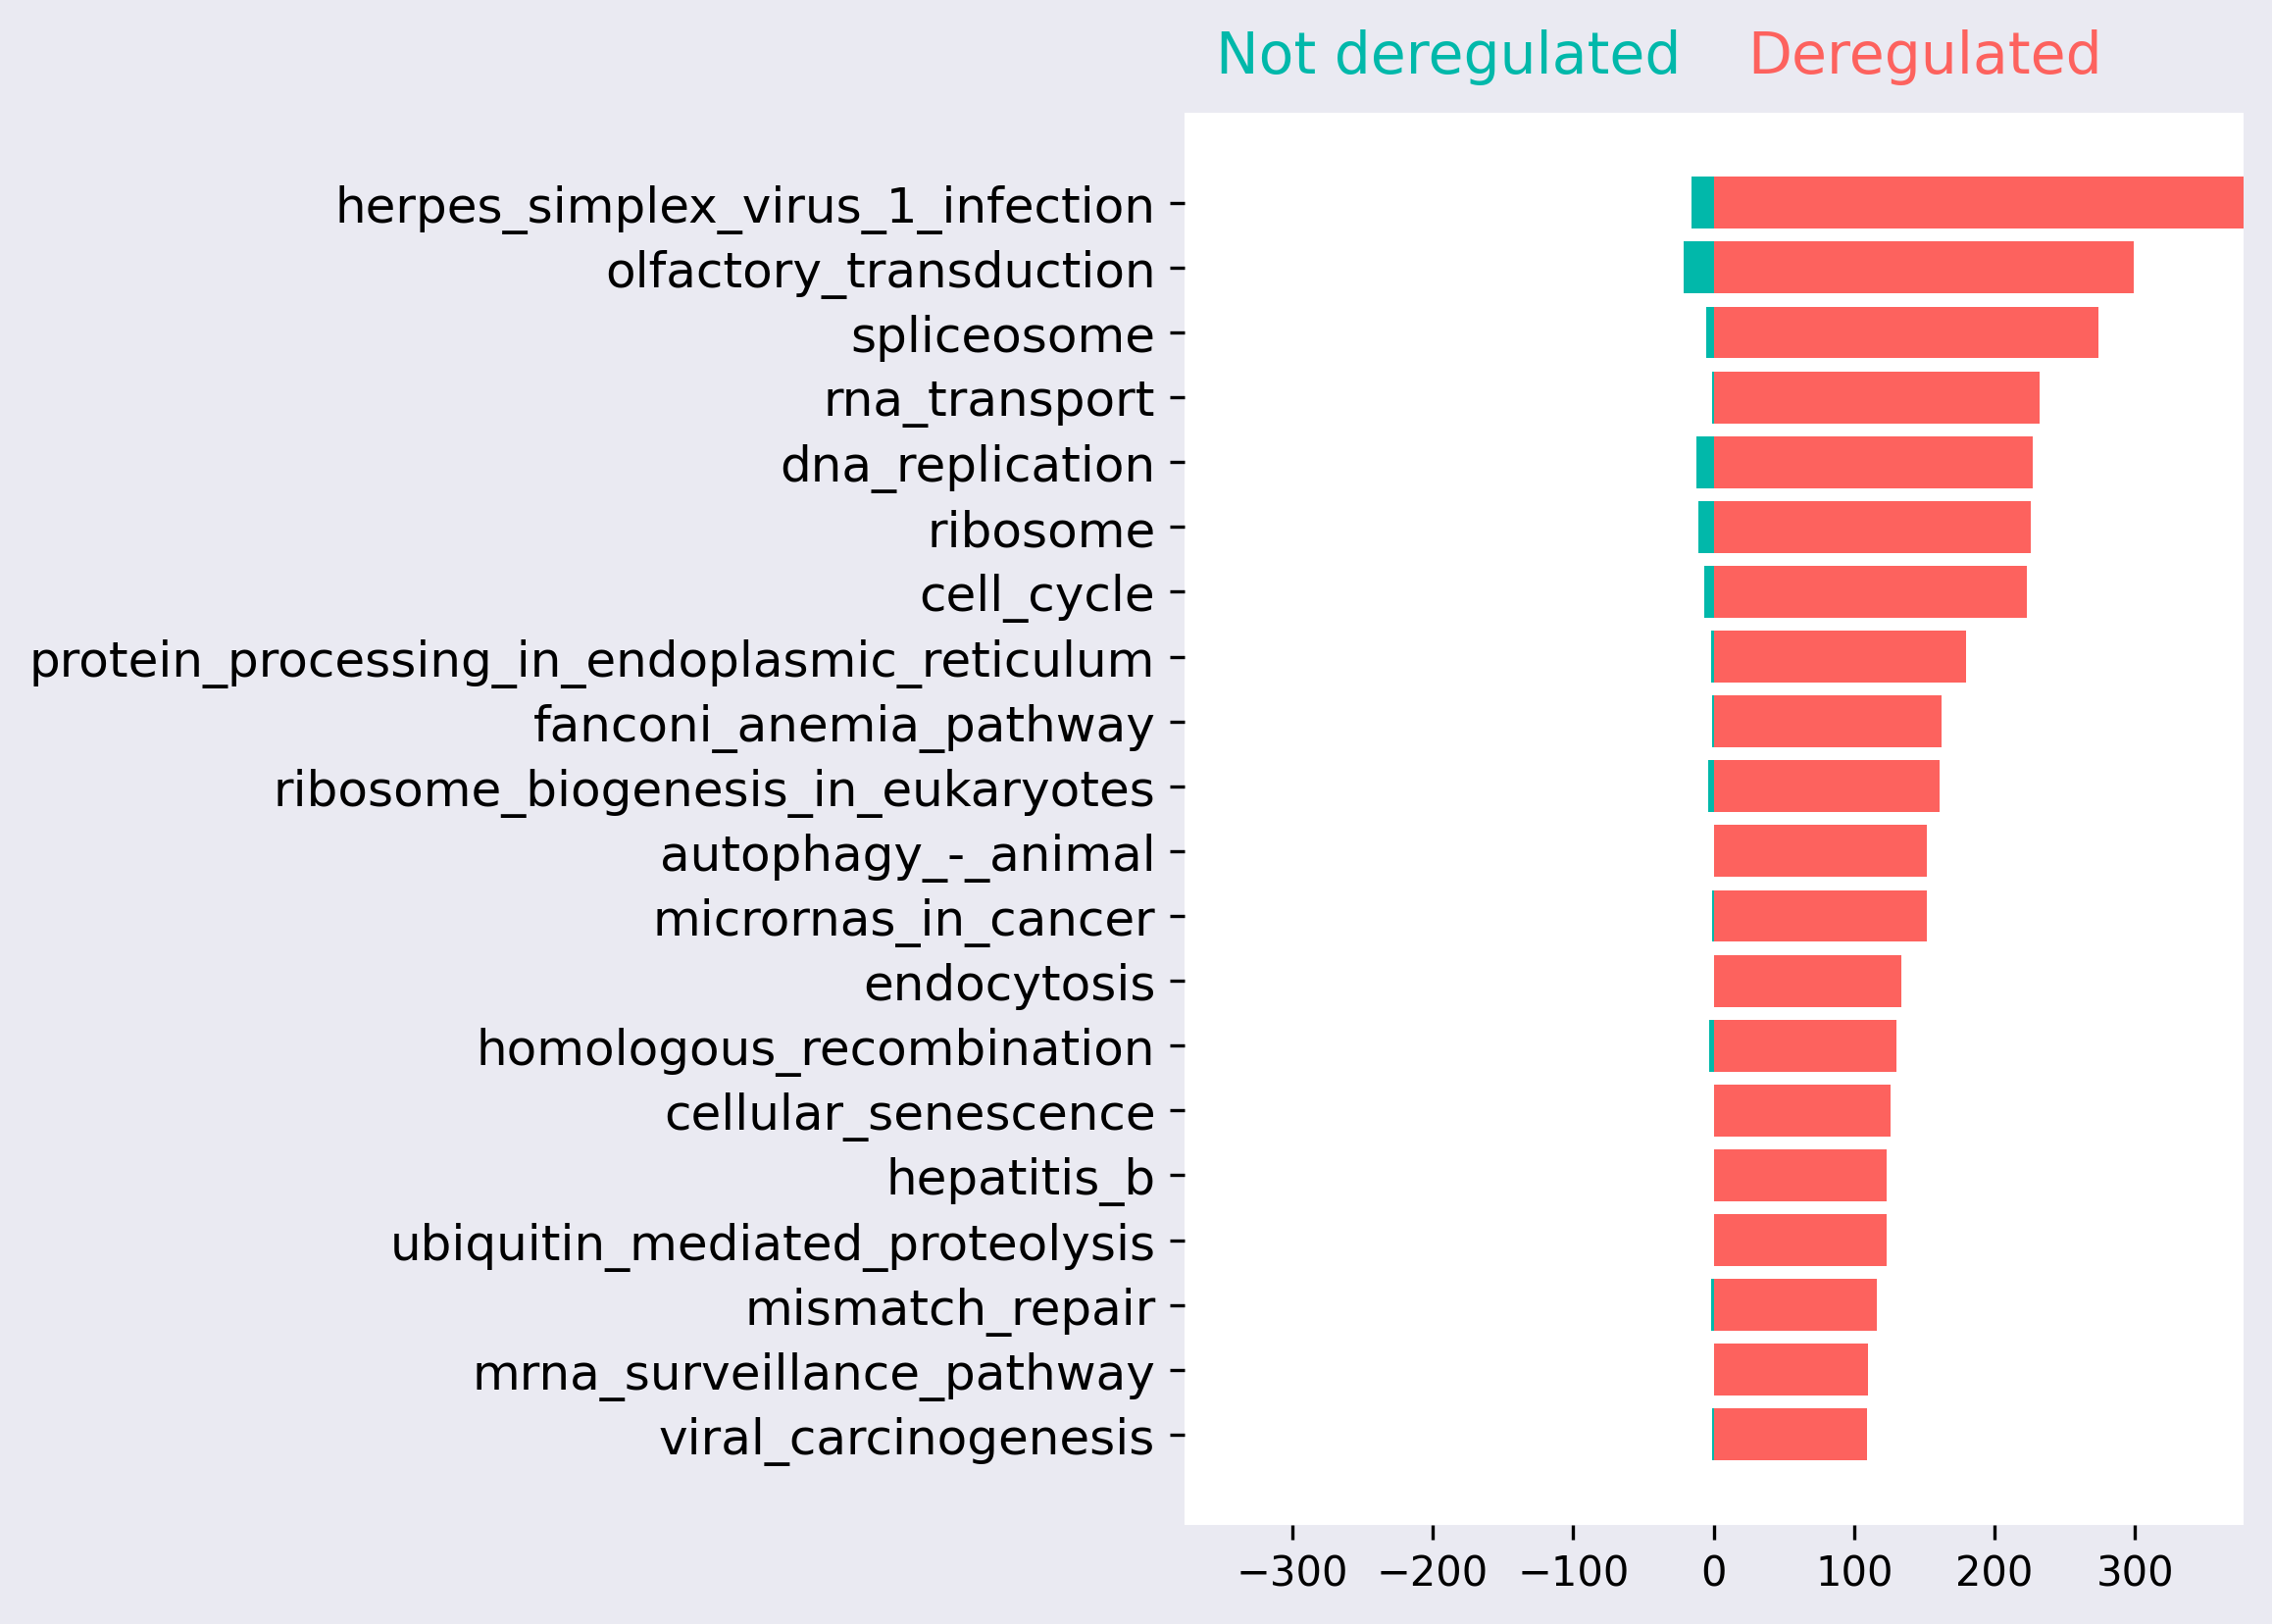
\includegraphics[width=0.8\textwidth]{bidir_bar_plot_enr2.png}
    \caption{Deregulated and not deregulated count, pathway-based gene expression enrichment\\deregulated and not deregulated count on x-axis, pathways on y-axis\\sorted by decreasing value of $\#_{\text{deregulated}}$\\gene expression values normalized with absolute $z$-scores, KEGG pathways}
    \label{fig:bidir_enr2}
\end{figure}
We suspect that, as has been found previously~\cite{transcription_translation_deregulation_cancer}, processes and pathways involved in gene expression (specifically transcription and translation) are going to be up-regulated in cancer cells. The pathways that were significant in our analysis support this hypothesis.\\
One pathway which was found to be significant in this analysis was the \textbf{spliceosome} pathway~\cite{kegg_spliceosome}. It was found to be significantly deregulated in $274$ cell lines with a median p-value of $0.00336$. The spliceosome is the entirety of the machinery managing the RNA splicing, which describes the post-processing of pre-mRNA after transcription. This mainly includes the removal of introns (sections that should not be translated). Even though the spliceosome is usually considered ``housekeeping'' machinery~\cite{spliceosome}, mutations and defects in it can still correlate to diseases, including cancer~\cite{spliceosome}. Therefore, the spliceosome has recently been considered as a potential target for new targeted cancer therapies~\cite{epigenetics_alternative_splicing}.\\
Another pathway which we deemed significant was the \textbf{RNA transport} or \textbf{nucleocytoplasmic transport} pathway~\cite{kegg_rna_transport}.  It was found significantly deregulated in $232$ cell lines with a median p-value of approximately $0.01276$. RNA transport, which describes the transportation of RNA from the nucleus to the cytoplasm between transcription and translation, is an essential part of gene expression, a process where cancer cells often differ from healthy cells~\cite{hallmarks-of-cancer}.
One of the main components of RNA transport is the Nuclear Pore Complex (NPC). It serves as the gateway for RNA and other macromolecules out of the cellular nucleus~\cite{npc_structure}. Perturbations in the function of the nuclear core complex have been associated with cancer formation~\cite{npc_structure}. Another molecule heavily involved in RNA transport are RNA helicases~\cite{rna_helicases}. During RNA transport, they take an important role in resolving RNA secondary structures, which are often just as essential to the correct translation or other function taken by the RNA as the base sequence itself~\cite{rna_secondary_structure}.
In 2013, Robert and Pelletier found alterations in the activity of RNA helicases to be implicated in the process of cancer formation~\cite{rna_helicases}. The deregulation of this pathway in cancer cells fits with their involvement with cancer. Kim et al.\ also found RNA-binding proteins to have an emerging role in cancer cells~\cite{rnabp_cancer}. RNA-binding proteins are an essential regulator of RNA transport~\cite{rnabp_cancer}, and alterations to their expression seem to play a major role in the development of cancer.\\
Next, we consider the \textbf{DNA replication} pathway~\cite{kegg_dna_replication}. It was significantly deregulated in $227$ cell lines with a median p-value of approximately $0.00173$. Since genomic instability is one of the most important and prevalent Hallmarks of Cancer~\cite{hallmarks-of-cancer}, potential defects and deregulation of the replication machinery being prevalent in cancer is to be expected. In 2015, Macheret and Halazonetis proposed DNA replication stress to be added as an additional hallmark of cancer~\cite{dna_replication_stress}. DNA replication stress refers to a condition where the typical DNA replication process in a cell is impeded. Oncogenes are able to induce DNA replication stress in a cell, leading them to provoke a stalling in the DNA replication. This is in contrast to what we might have expected: as mentioned previously, cell cycle processes (including DNA replication) tend to be up-regulated in cancer cells, to facilitate a quick growth of the cancer. While the exact mechanisms on how this happens have not been explored clearly, a link between DNA replication stress and oncogenesis is supported by literature. The deregulation of DNA replication can easily facilitate the genesis of DNA replication stress.\\
The \textbf{cell cycle} pathway~\cite{kegg_cell_cycle} was also found significantly deregulated in our analysis. It was deregulated in $223$ cell lines with a median p-value of approximately $0.00170$. This pathway controls the cell cycle in general, including DNA replication and mitosis. Deregulations and other abnormalities in the cell cycle have long been known as being very common in cancer cells. For instance, Todd et al.\ found the dysregulation of the cell cycle to be emerging as a central theme of carcinogenesis in oral cancer. This is, however, only one example case, as cell cycle deregulation is known as a tumor marker in general. It is closely linked to several Hallmarks of Cancer~\cite{hallmarks-of-cancer}, namely the self-sufficiency in growth signals, the insensitivity to anti-growth signals and the limitless replicative potential. All these hallmarks are defects to processes that would typically be tightly regulated in regards to the cell cycle. Cell cycle checkpoints, which are usually points where errors in the cell cycle progresses are detected, but are often deregulated or defective in cancer cells, have also been considered as potential targets for targeted anticancer therapy~\cite{cell_cycle_dysregulation_anticancer}.\\
Lastly, the \textbf{miRNAs in cancer} pathway was also identified to be significantly deregulated. It was deregulated in $152$ cancer cell lines, and the median p-value was approximately $0.0173$. MicroRNAs (miRNAs) are short (around $20$ nucleotide) non-coding RNA strands, that have a multitude of mostly regulatory roles around the cell.\@
miRNA dysregulation has often been observed in many cancers~\cite{mirna_dysregulation_cancer}. Therefore, a link to carcinogenesis has been hypothesized~\cite{mirna_dysregulation_cancer} and miRNAs have also been considered as potential targets for targeted cancer therapies~\cite{mirna_targeted_cancer_therapy}.
%miRNA dysregulation has also been found\addref{Source!} to have consequences on pathways which lead to carcinogenesis, and have therefore been also handled as potential targets for new targeted cancer therapies.
%One pathway which was found significant in this analysis was the \textbf{neuroactive ligand-receptor interaction} pathway~\cite{kegg_nlri}. This pathway handles environmental information processing through signaling molecules and the interaction with them. It was found to be significant in $762$ cell lines with a median p-value of approximately $0.00063$. In a 2023 article by Yang et al., they attempted to find an underlying mechanism to explain the association between homologous recombination deficiency (HRD) in colon cancer (which is a defect in one of the most important and reliable DNA repair pathways, namely homologous recombination). They found that the neuroactive ligand-receptor interaction pathway was overexpressed in tumors with high HRD, as well as associated with resistance to immunotherapy by way of immunosuppression in colon cancer. This shows that the expression of this pathway was previously already found to be altered in cancer cells, which is coherent with our result.\\
%Another significant pathway was the \textbf{tyrosine metabolism} pathway~\cite{kegg_tyrosine_metabolism}, which was found significant in $254$ cell lines with a median p-value of approximately $0.0248$. Tyrosine is an amino acid, the phosphorylation of which is an essential post-translational modification to promote the metabolic reprogramming of cancer cells~\cite{tyrosine_phosphorylation}. Since it plays a fundamental role in cancer development, we could hypothesize that it also influences drug sensitivity.\\
%The next significant pathway in our analysis was the \textbf{retinol metabolism} pathway~\cite{kegg_retinol_metabolism}. This pathway is responsible for the metabolism of retionids (vitamin A derivatives). It was found significant in $354$ cell lines with a median p-value of approximately $0.013$. In a 2010 article, Bushue and Wan highlighted the potential use of retinoids (e.g. retinoic acid, which is a metabolite of retinol) as anti-cancer medication, since they show ``anti-proliferative, pro-apoptotic, and anti-oxidant effects''~\cite{retinoid_pathway_cancer}.\\
%The \textbf{viral protein interaction with cytokine and cytokine receptor} pathway~\cite{kegg_cytokine_interaction} was found significant in $690$ cell lines with a median p-value of approximately $0.0043$. Cytokines are soluble small polypeptides or glycoproteins secreted by immune cells, that act as signaling molecules to regulate and coordinate immune responses. Anti-inflammatory cytokines have been found to be important in regulation of inflammatory response. A disrupted balance between pro- and anti-inflammatory mechanisms can lead to chronic immune activation and inflammation, as is often observed in people with cancer~\cite{cytokines_cancer}. Viruses have evolved into copying host cytokines and cytokine receptor genes, to produce their own cytokine-binding or cytokine receptor-binding proteins, in the pursuit of evading immune response~\cite{kegg_cytokine_interaction}.\\
%Another pathway of interest, resulting from this enrichment analysis, was the \textbf{chemical carcinogenesis} pathway\addref{there are multiple ``chemical carcinogenesis'' PWs in KEGG!}. This describes the process in which cancer formation is triggered by exposure to toxic chemical compounds. The pathway outlines the process by which this can happen, including the metabolism of xenobiotics (foreign compounds), which converts them into highly reactive compouds. Those compounds can then attack and damage DNA and other cell-interal structures, which can lead to a cell becoming cancerous~\cite{chemical_carcinogenesis}.\\
%Finally, the last significant pathway discussed will be the \textbf{Drug metabolism --- cytochrome P450} pathway~\cite{kegg_cytochrome_p450}. This pathway has been found to be involved in the metabolism of a variety of cancer drugs by Fujita et al.\ in 2006~\cite{cytochrome_p450}. Therefore, it being differentially expressed in cancer cells is consistent with previous knowledge about this pathway.

\subsection{Pathway-based Drug Sensitivity Enrichment}\label{subsec:bidir_enr3}
In our third and final enrichment analysis, we used the categories generated based on the results from the previous enrichment (namely, cell lines in which a certain pathway is deregulated) in tandem with the drug sensitivity values previously used in the first enrichment, in the aim to find associations between altered pathways and increased drug sensitivity or resistance to specific drugs.\\
For this enrichment, we count for how many different drugs this specific pathway is associated with significantly increased sensitivity or resistance.\\
\begin{figure}
    \centering
    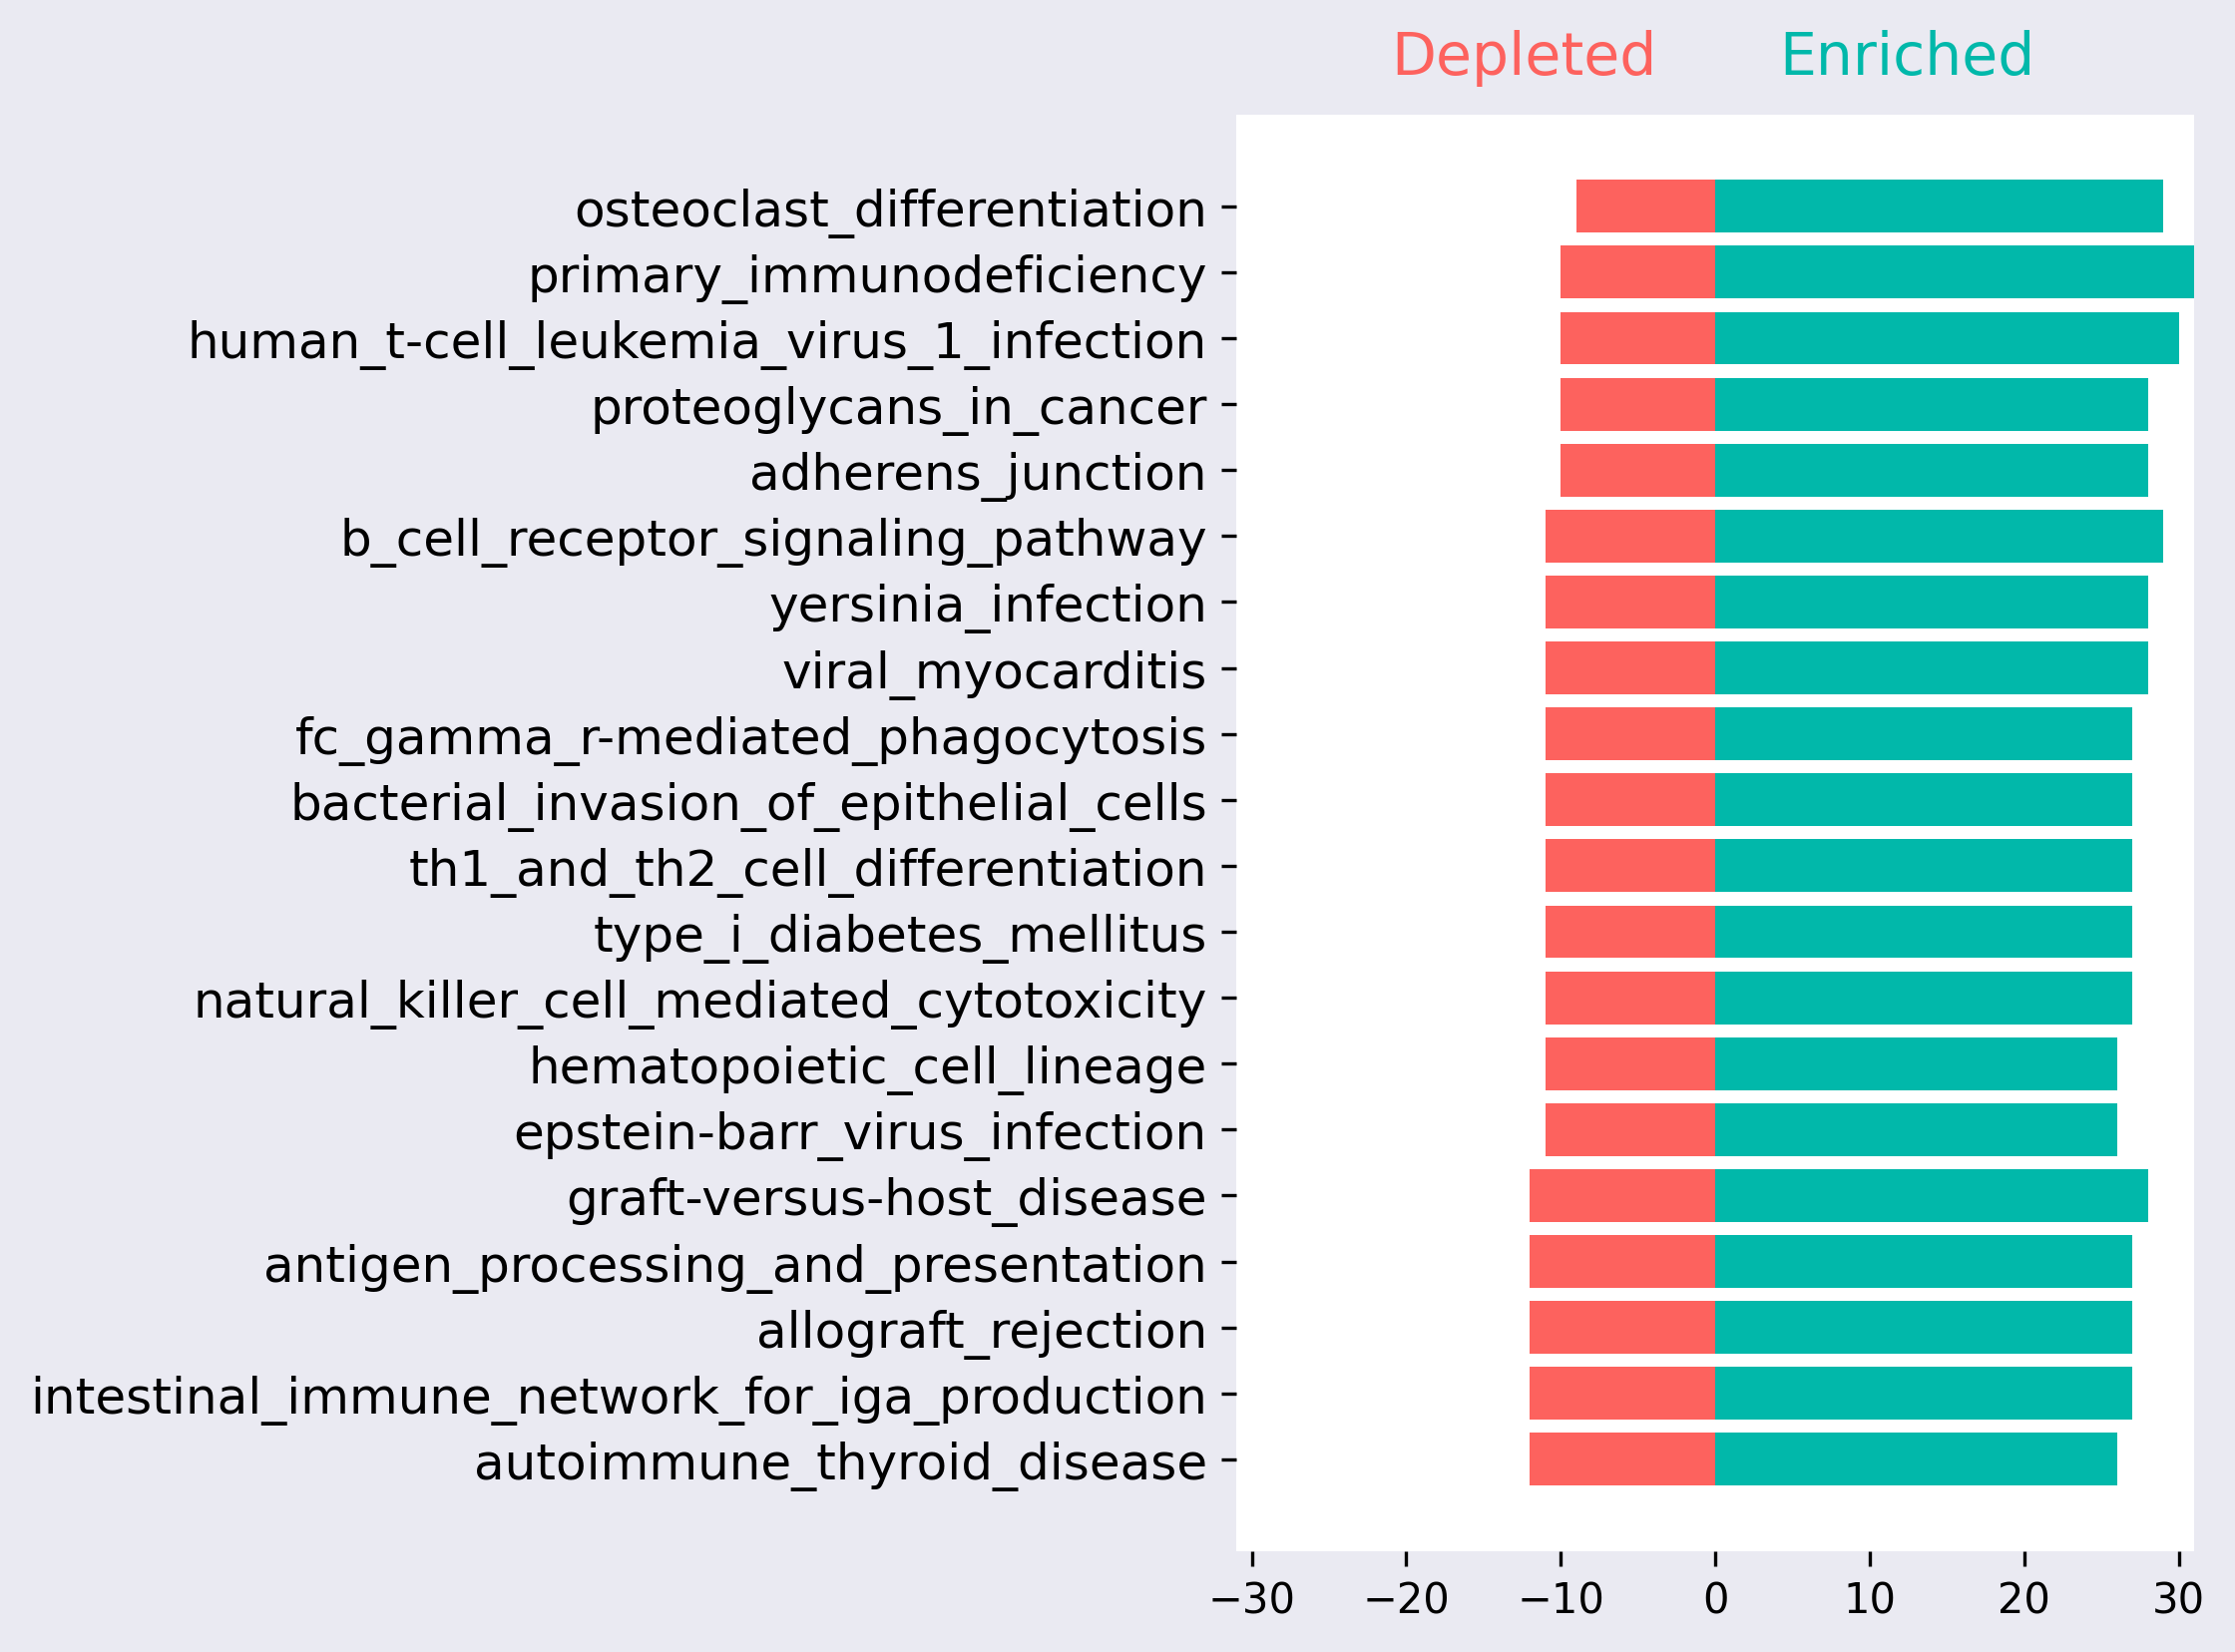
\includegraphics[width=0.8\textwidth]{bidir_bar_plot_enr3.png}
    \caption{Count of enriched and depleted pathways in the gene-based drug sensitivity enrichment analysis. Count of enriched and depleted pathways on $x$-axis, pathways on $y$-axis. Sorted by decreasing value of $\frac{\#_{\text{enriched}}}{\#_{\text{depleted}}}$.\\Dataset: GDSC2, drug sensitivity: CMax-Viability\\The negative numbers for depleted are only there for technical reasons and still describe only the count.}
    \label{fig:bidir_enr3}
\end{figure}
One of the pathways which turned out to be enriched the most often is the \textbf{primary immunodeficiency} pathway~\cite{kegg_pid}. Primary immunodeficiencies (PIDs) are a heterogeneous group of diseases, which affect the immune system (mainly the non-specific immune response), creating a susceptibility to infection and malignancies. More specifically, the primary immunodeficiency pathway in the KEGG database describes the differentiation of T and B cells. PIDs have been found to severely complicate cancer treatment by provoking serious toxicities as a long-term effects~\cite{pids, pid_cancer}, inducing secondary malignancies. In the context of a tumor, PIDs can modify the tumor microenvironment and weaken the immune system in general, which aids tumors to proliferate. Aside from that, they severely increase the risk for side effects, since patients with PIDs are severely more prone to infections, which can also increase adverse effects from cancer drugs.
Therefore, it is reasonable that a deregulation of this pathway would be associated with an increased drug sensitivity in cancer cell lines (cf. Figure~\ref{fig:bidir_enr3}). Since we do not know anything about the regulation direction of that pathway, we can hypothesize that its activity would be decreased. Generally, we would assume that the down-regulation of this pathway might lead to increased drug sensitivity, while its down-regulation might lead to increased resistance, but our analyses can neither confirm nor deny this claim.\\
Another pathway of which the deregulation is significantly associated with an increased sensitivity against cancer drugs is the \textbf{B-cell receptor signaling pathway}~\cite{kegg_b_cell_receptor_signaling_pathway}. This pathway was identified as a potential target pathway for cancer mediation~\cite{b_cell_receptor_signaling_pathway}. It is indispensable for normal B cell development, which together with macrophages, can be part of a tumor-supportive microenvironment in solid tumors~\cite{b_cell_receptor_signaling_pathway}. This pathway is also sometimes used by malignant B cells in leukemias and lymphomas (fluid tumors). Therefore, this pathway being deregulated in sensitive cell lines aligns with previous literature.\\
Finally, the \textbf{FC-$\gamma$ receptor-mediated phagocytosis}~\cite{kegg_fc_gamma} pathway was found to be significantly associated with increased drug sensitivity. In a 2020 paper, Qian et al.~\cite{fc_gamma} identified around 1000 SNPs (single nucleotide polymorphisms) in genes of this pathway to be related to lung cancer survival. This pathway was also found to have altered expression in some cancers, and it is suspected that the human anti-cancer antibodies IgG1 and IgG3 could interact with some FC-$\gamma$ receptors~\cite{fc_gamma_cancer}.

\section{Drug-specific Analysis of Rapamycin}\label{sec:rapamycin_analysis}
To show how our methodology could be used to identify potential biomarkers, such as genes or pathways which might be associated with an increased sensitivity or resistance to one specific drug, we focused on \textbf{Rapamycin} as an exemplary drug. We identified genes and pathways that our analysis found to be significant, and considered whether they had a link to Rapamycin sensitivity which could be explained from biological literature.\\
Rapamycin is a specific inhibitor of the mTOR (mammalian target of Rapamycin) pathway~\cite{kegg_mtor}, which is a ``master regulator of cell growth and metabolism''~\cite{rapamycin_one_drug_many_effects}. It suppresses immune responses and has been identified as a key regulator of pathways often found to be deregulated in cancer cells~\cite{mtor_cancer}. Consequently, there has been increasing focus on rapalogs (Rapamycin analogs) and other mTOR inhibitors in cancer therapy, due to their potential to target deregulated pathways in oncology~\cite{towards_rapalog_cancer_therapy}.\\
Again, we limit ourselves to the GDSC2 dataset and the CMax-Viability as a drug sensitivity measure for the purpose of these following analyses. This gives us a dataset comprising $741$ cell lines.

%Rapamycin is a specific inhibitor of the mTOR (mammalian target of Rapamycin) pathway, which is a ``master regulator of cell growth and metabolism''~\cite{rapamycin_one_drug_many_effects}. It suppresses immune responses and has been identified to be a key regulator of pathways often found to be deregulated in cancer cells~\cite{mtor_cancer}. Consequently, the potential uses of rapamycin in oncology and mTOR-targeted cancer therapy have been playing an increasingly large role in oncology, focusing on rapalogs (Rapamycin analogs) and, later, also on alternative mTOR inhibitors~\cite{towards_rapalog_cancer_therapy}.

\subsection{Significant Genes}\label{subsec:rapamycin_genes}
For the first enrichment analysis, which identified significant genes, we focused on three genes which were found to be significant.\\
%The GDSC2 dataset brings great improvements over GDSC1 according to the creators of the GDSC database. Also, the CMax-Viability provides some advantages over the typically used IC50 value, and is a rather new and unexplored measure of drug sensitivity, which is why we chose to focus on it for this experiment.\\
The first gene which was found to be significant was \textbf{CtBP2} (Carboxyl terminal-binding protein 2). It was found to be significantly associated with increased drug resistance when down-regulated with a p-value of $2.8488\times10^{-5}$. It encodes a transcriptional corepressor, which regulates gene expression by binding to other transcription factors, repressing genes involved in cell differentiation, apoptosis and cancer progression~\cite{ctbp2_transcriptional_corepressor}. It is associated with supporting cell survival and growth in cancer~\cite{ctbp2_transcriptional_corepressor}. The gene was also found to suppress the \emph{focal adhesion-PI3K-Akt-mTOR}-signaling pathway, which is also a target for Rapamycin~\cite{ctbp2_mtor}. With this knowledge, a gene which down-regulates the target pathway of Rapamycin being associated to an increased resistance to that drug is a coherent result, since the down-regulation of the CtBP2 gene would lead to a lower baseline activity of the mTOR pathway, making the inhibitory impact of Rapamycin on the pathway smaller, which can reduce the sensitivity.\\
Another significant gene was \textbf{FAM129B} (Family with sequence similarity 129, member B). It was found to be significantly associated with increased drug resistance when down-regulated with a p-value of $8.6829\times10^{-7}$. FAM129B is a suppressor of the TNF-$\alpha$ apoptotic pathway~\cite{fam129b}. It has also been found to promote a survival pathway in cancer~\cite{fam129b}. Firstly, we can already say that, without referring to Rapamycin specifically, a gene which suppresses apoptosis (which is one of the principal ways the organism fights cancerous cells) and promotes a survival pathway in cancer being linked to a reduced drug sensitivity is coherent, since it increases the overall survival chances of the cancer. More specifically referring to Rapamycin, we know that Rapamycin is also an inhibitor of the specific TNF-$\alpha$ pathway which is suppressed by FAM129B~\cite{tnfalpha}. In a similar argument to the previous paragraph, this is indeed coherent.\\
One more gene to be deemed significant was \textbf{Myo1b} (Myosine 1 b). It was found to be significantly increasing drug resistance when down-regulated with a p-value of $8.6829\times^{-7}$. It encodes the Myosin 1b protein, which functions as a molecular motor protein~\cite{myo1b_function}. It also plays a pivotal role in autophagy, of which mTOR is a key regulator. The link here is not quite as apparent as for the previous genes. Autophagy is a way for the cell to degrade damaged or superfluous proteins and organelles. In tumour cells, which often have defects in apoptosis, autophagy can allow for prolonged survival of the cell~\cite{autophagy_cancer}. Since Myo1b plays a pivotal role in autophagy~\cite{myo1b}, and mTOR is also a pivotal regulator of the autophagy process~\cite{mtor_autophagy}, Myo1b being associated with an altered drug sensitivity seems also reasonable.

\subsection{Significant Pathways}\label{subsec:rapamycin_pathways}
Similarly to the previous analysis of genes, we also analyzed the results of the pathway-based drug sensitivity enrichment to identify pathways that might be especially linked to an increased sensitivity or resistance to Rapamycin.\\
A highly interesting and desirable result would have been to find the \textbf{mTOR} (mammalian target of Rapamycin) pathway itself to be associated to a change in the sensitivity to Rapamycin. Unfortunately, this was not the case, as the mTOR pathway was only found with a p-value of approximately $0.37$. There are different potential explanations for this: while mTOR is the target pathway of Rapamycin, it is part of a highly complex signaling network, being a key regulator of many other pathways~\cite{rapamycin_multi_faceted}. Also, mTOR was found to be involved in a negative feedback loop by Carracedo et al.\ in 2008~\cite{mTOR_negative_feedback_loop}, where cells were able to circumvent the effect of Rapamycin by activating alternative cell signaling pathways.\\
We did, however, find some pathways which were significant in regards to the sensitivity to Rapamycin, and which can be explained by previous literature. One of these was the \textbf{Intestinal immune network for IgA production} pathway~\cite{kegg_iga}. The deregulation of this pathway can be linked to an increased sensitivity to rapamycin with a p-value of approximately $0.0092$. The intestine plays a major role in immune response, since it has the ability to produce large quantities of the noninflammatory IgA (immunoglobin A) antibodies, which serve as the first line of defense against microorganisms. The deregulation of a pathway which produces noninflammatory antibodies fits with an increased sensitivity to Rapamycin, since Rapamycin itself has shown potential as an antiinflammatory drug~\cite{rapamycin_multi_faceted}.\\
Another pathway which was found to be significant in relation to the sensitivity to Rapamycin was the \textbf{hematopoietic cell lineage} pathway~\cite{kegg_hematopoietic_cell_lineage}, which was linked to an increased sensitivity to Rapamycin with a p-value of approximately $0.00438$. As it turns out, the mTOR pathway is an important regulator of hematopoietic stem cell renewal~\cite{mtor_hematopoietic}. The pathway controls the processes of differentiation, where hematopoietic stem cells differentiate into blood cells through several intermediate steps. Since mTOR is also a key regulator of this process, the literature supports this association.\\
The final pathway which we found to be significantly associated with Rapamycin resistance is the \textbf{Cell Adhesion Molecules (CAMs)} pathway~\cite{kegg_cam}. It had a p-value of approximately $0.00920$. CAMs are membrane proteins, some of which are responsible for cell adhesion. In a 2016 paper, Solthibundhu et al.\ found that 3 target genes of Rapamycin modulate the dynamics of the actin skeleton, which is critical for cell adhesion, among other things~\cite{rapamycin_cell_adhesion}. This highlights a potential link between the effect of Rapamycin in a cell and the considered pathway.

\section{Principal Component Analysis}\label{sec:pca}
Principal component analysis (PCA)~\cite{jolliffe_pca} is a technique for dimensionality reduction, used for the simplification of complex datasets, while still capturing as much of the original variance as possible.\\
In our analyses, similarly to lots of bioinformatics problems, the dimensionality of our results can be extremely large. That makes the interpretation of these datasets very hard for humans. By reducing the dimensionality using PCA, we make the dataset more interpretable through using visualization techniques like scatter plots.

We performed a PCA on the results of the pathway gene expression enrichment. The results of the enrichment analysis consisted of p-values for every combination of pathway and cell line, as well as a regulation direction, indicating how much the pathway is up- or down-regulated in that specific cell line. These values were converted into a matrix, containing the p-value for each combination of $334$ pathways and $1014$ cell lines. The p-values were normalized through a $\log_{10}$ calculation. The regulation direction result was also encoded into the p-values, by making them positive for deregulated and negative for not deregulated pathways. The dimensionality of pathways in this matrix was reduced from 334 to 2. Then, a scatterplot was again created. The individual dots, each representing a cell line, were colored according to the cancer histology of that specific cell line. The plot can be seen in Figure~\ref{fig:pca_enr2}.\\
\begin{figure}
    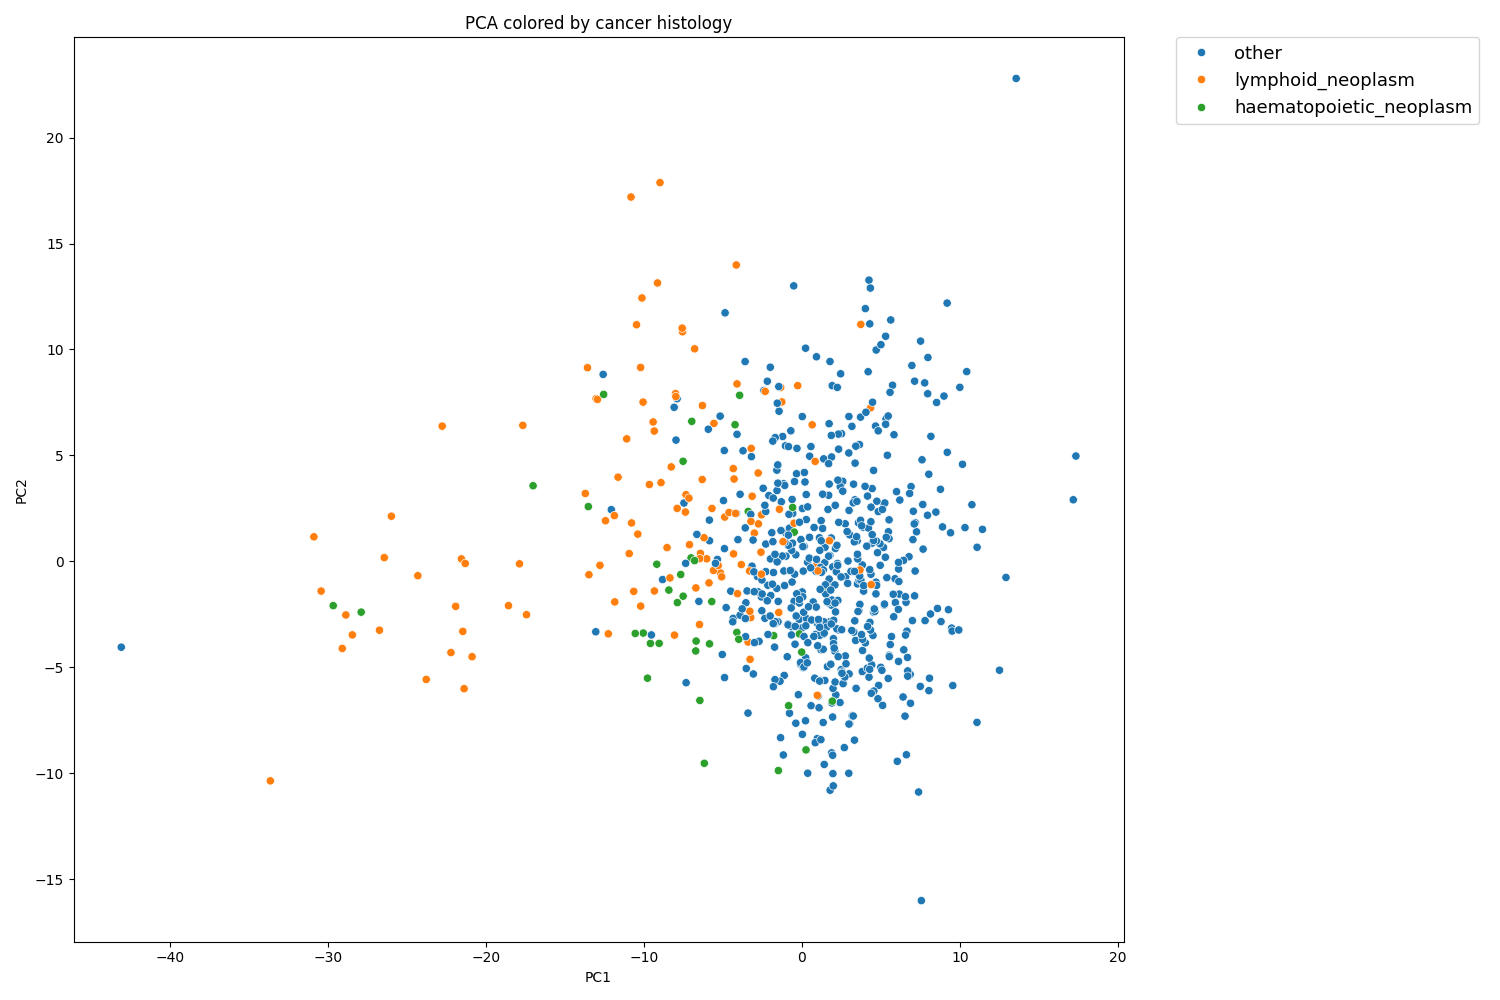
\includegraphics[width=\textwidth]{pca_results_absolute_zscores_hists.png}
    \caption{PCA scatterplot\\resulting p-values of pathway gene expression enrichment\\after reducing the dimensionality of the pathways to $2$\\every dot represents a cancer cell line, colored by histology}
    \label{fig:pca_enr2}
\end{figure}
%Evidently, that is an unmanageable number of p-values to manually interpret.
We can, see a certain separation between the \textbf{lymphoid neoplasm} and \textbf{hematopoietic neoplasm} histologies, and the rest of the categories. These two categories were selected specifically, since they represent the liquid tumors, as opposed to solid tumors growing in one locus. Due to the very different environment and conditions faced by liquid tumors in contrast to solid tumors, a difference in their gene expression is to be expected.
%Since these two categories represent fluid tumors (in the blood or lymph), as opposed to solid tumors, growing on other organs.
%To summarize, we observed a difference in gene expression of pathways between solid and fluid tumors, which seems very coherent, as the conditions faced by the tumors in their respecitve environment differ very strongly between solid and fluid tumors.\\
%When coloring the same PCA plot by cancer site instead of histology, we found an analogous separation between cancers in the \textbf{hematopoietic and lymphoid tissue} and other tumors. Similarly to before, we focused on the enrichment analysis done on absolute z-scores for this PCA.\@The PCAs for the enrichment based on pure gene expression values and z-scores, respectively colored by cancer site and cancer histology, can be found in the appendix\todo{add plots into appendix}.

We then performed a PCA analysis on a matrix of CMax-Viability drug sensitivity values, for $42$ drugs and $600$ cell lines. We reduced the dimensionality of the drugs to 2 and created a scatterplot, again coloring the cell lines by their cancer histology. Again, we limited to ourselves to considering the histologies of liquid tumors. Since we already observed a difference in gene expression between liquid and solid tumors, we wanted to find out whether there is also a difference in drug sensitivity. The PCA scatterplot can be seen in Figure~\ref{fig:pca_cmax}.
\begin{figure}
    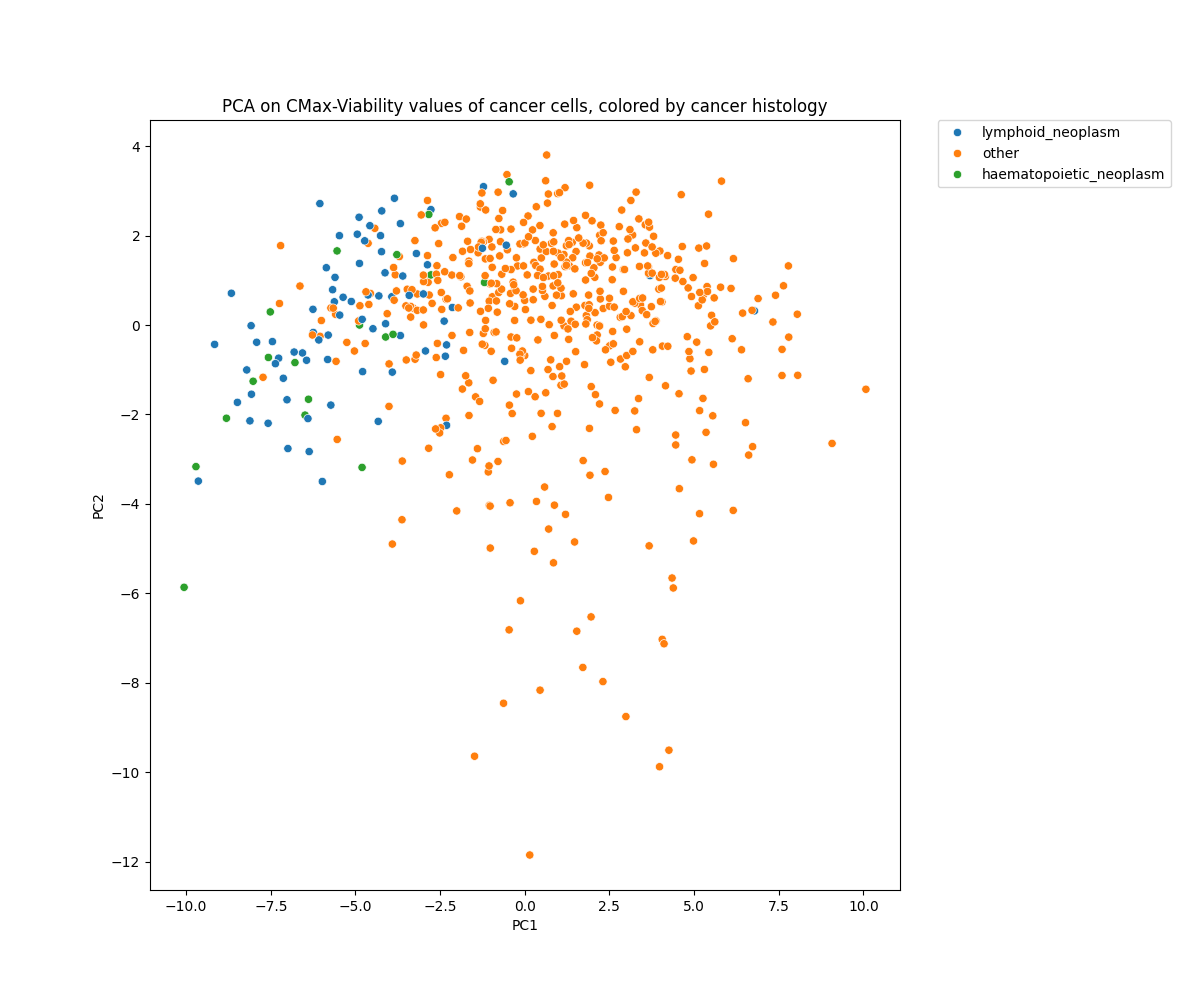
\includegraphics[width=\textwidth]{PCA_CMax_Matrix.png}
    \caption{PCA scatterplot\\CMax-Viability matrix\\after reducing the dimensionality of the drugs to $2$\\every dot represents a cancer cell line, colored by histology}
    \label{fig:pca_cmax}
\end{figure}
We can, again, see that the two highlighted histologies of \textbf{lymphoid neoplasm} and \textbf{hematopoietic neoplasm} separate quite clearly from the rest of the histologies. This allows us to support the fact that fluid tumors (in the blood or lymph) often tend to exhibit a stronger drug sensitivity than solid tumors (which are growing in one place in an organ), which has been observed previously~\cite{fluid_solid_tumors_sensitivity, tissue_specificity_of_in_vitro_drug_sensitivity}.\\
PCA analyses were also performed on the results of the gene-based drug sensitivity enrichment. However, no interesting seperation was noted. The corresponding scatter plots are provided in \hyperref[appendix:pca]{Appendix B}.

%\section{Pathways of interest}
%\textsc{Will I even need this? What pahtways should this be about?}

%\section{Gene-based drug sensitivity enrichment}
%\subsection{Using IC50 values}
%Different\remove{Beschreibung der Enrichments ist jetzt in SD\&I, hier wirklich nur Ergebnisse} visualisations were performed to interpret the results of this enrichment. A PCA was performed, where in the gene expression alteration $\times$ cell line matrix created from the PCA results, the dimensionality of the gene expression alterations was reduced to 2, so that values can be visualized in a 2-dimensional scatter plot. The scatter plot, with each dot corresponding to a cell line, was colored by the respective site and histology of that cancer cell line. Unfortunately, no interesting separation could be noted in the scatter plot.\\
%\subsection{Using CMax-Viability values}
%The same enrichment was done again, only this time, using CMax-Viability values instead of IC50 values.\\
% As introduced earlier, the CMax-Viability value measures drug response in a similar fashion to the IC50 value. \todo{PCA erwähnen? Ergebnisse interessant? Evtl Vergleich zwischen IC50 und CMax-Viability Ergebnissen}

%\section{Pathway gene expression enrichment}
%As previously described, an enrichment based on gene expression values and pathways was performed. On the results of that enrichment analysis, a PCA was used to reduce the dimensionality of the dataset to $2$, the result of which was then plotted in a multi-colored scatter plot.\\
%With the resulting plot for the histology coloration~\ref{fig:pca_exp_site}, it can be seen that the gene expression profiles (which is what the PCA ultimately reduced to a dimensionality of $2$2) of fluid tumors is strongly separate and distinct from those of solid tumors. This is very coherent information, since the gene expression for fluid tumors (e.g. which reside in the blood or lymphous systems in the body) will differ strongly from that from solid tumors (which usually attach to a surface inside the body, need to form a ) due to the different micro-environment it is subject to.\\
%When performing the same PCA, but coloring the plot by cancer histology, gives a similar results: here, the categories clearly separating themselves from he rest are two, namely ``lymphoid neoplasm'' and ``haematopoietic neoplasm'', which precisely mirror the fluid tumors which are highlighted in the site coloring. The corresponding plot can be found in the appendix.\todo{really?}\\
%It is also important to note that, when normalizing the expression values first by calculating z-scores before performing the enrichment, the separation does not occur.\todo{investigate.}\\
%\begin{figure}
%    \centering
%	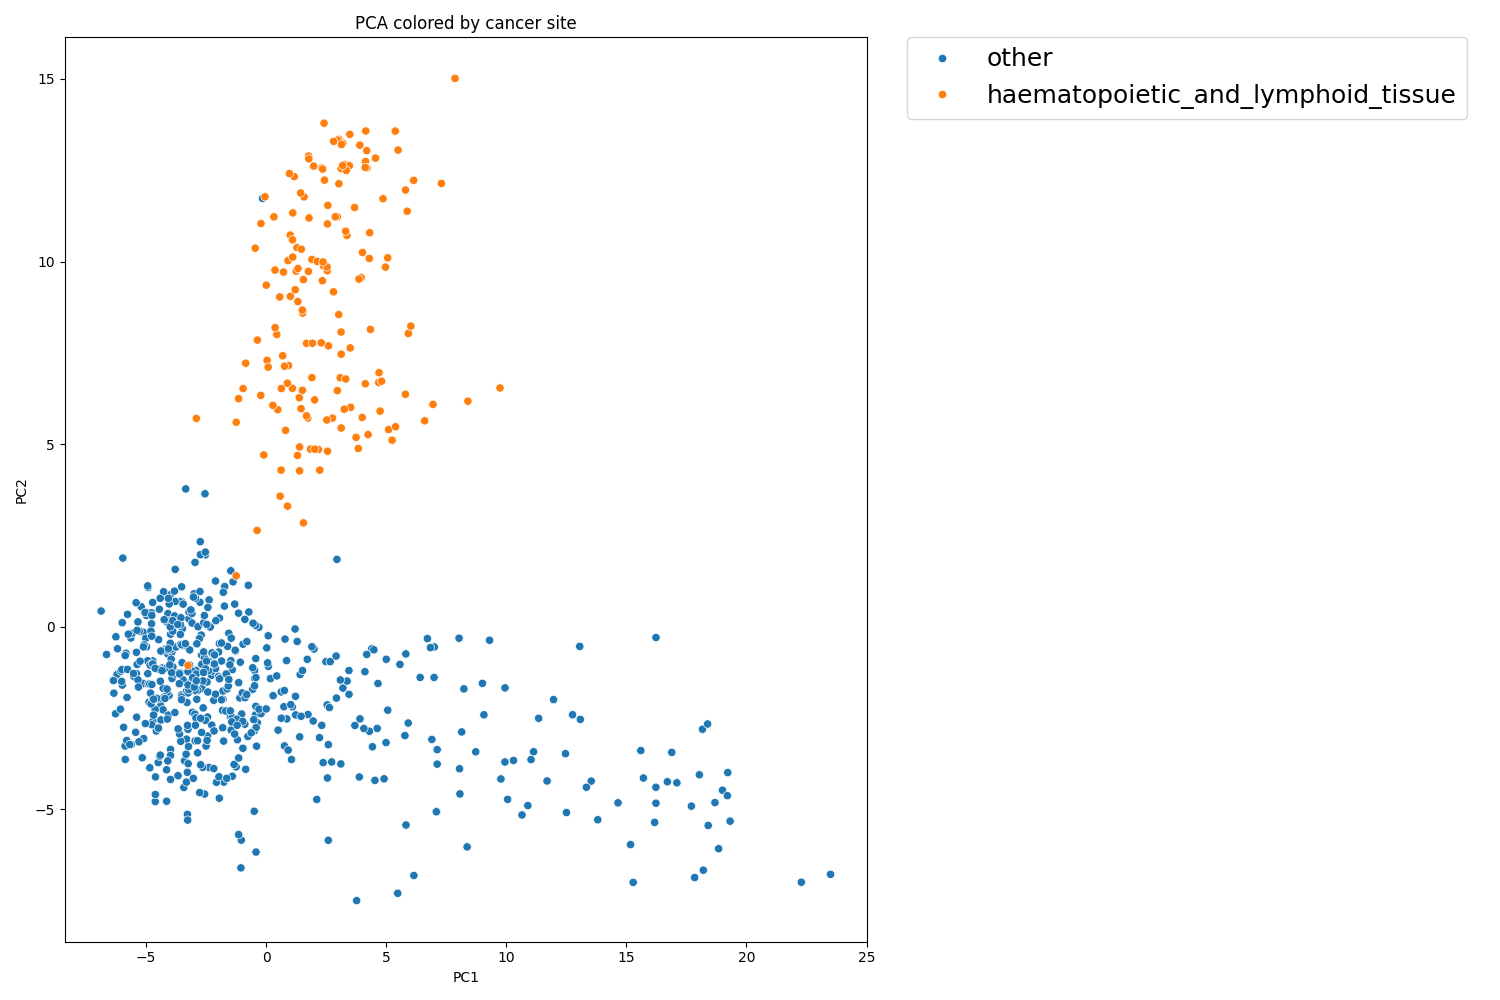
\includegraphics[width=0.7\textwidth]{pca_results_expression_values_site.png}
%	\caption{PCA result on the enrichment results using expression values, colored by cancer site}
%	\label{fig:pca_exp_site}
%\end{figure}
%The result of this analysis, while not very interesting in itself, can provide great categories for the next enrichment, as it optimizes the categories in the original enrichment. Instead of using individual genes that are abnormally up- or down-regulated, we use pathways, which is a much more interesting consideration for obvious reasons.\\


%\section{Pathway-based drug sensitivity enrichment}
%Finally, an improved version of the original first enrichments was performed on both the IC50 and CMax-Viability input values. As previously described, the categories were replaced: while the previous enrichment only used over- or under-expression of individual genes calculated from gene expression data as categories, this new enrichment used the over- or underexpressed pathways provided by the result of the second enrichment as categories. This is a much more informative analysis, as individual genes being over- or under-expressed might not have a strong or clearly interpretable biological meaning, while the function of biological pathways is much more describable and well-known, so their enrichment or depletion can give much more informative results.\\
%For this enrichment, a script counting the total number of significantly enriched or depleted categories (in this case, pathways) for every cell line was used. This was plotted as a bidirectional bar plot, with the number of enrichments and depletions being plotted for every pathway.\\
%\textsc{find out if there are any specific pathways that tend to be enriched or depleted in most cases.\\ Note: enrichment of up-regulation of pathway is the same as depletion of down-regulation}